\documentclass[twoside]{book}

% Packages required by doxygen
\usepackage{fixltx2e}
\usepackage{calc}
\usepackage{doxygen}
\usepackage[export]{adjustbox} % also loads graphicx
\usepackage{graphicx}
\usepackage[utf8]{inputenc}
\usepackage{makeidx}
\usepackage{multicol}
\usepackage{multirow}
\PassOptionsToPackage{warn}{textcomp}
\usepackage{textcomp}
\usepackage[nointegrals]{wasysym}
\usepackage[table]{xcolor}

% Font selection
\usepackage[T1]{fontenc}
\usepackage[scaled=.90]{helvet}
\usepackage{courier}
\usepackage{amssymb}
\usepackage{sectsty}
\renewcommand{\familydefault}{\sfdefault}
\allsectionsfont{%
  \fontseries{bc}\selectfont%
  \color{darkgray}%
}
\renewcommand{\DoxyLabelFont}{%
  \fontseries{bc}\selectfont%
  \color{darkgray}%
}
\newcommand{\+}{\discretionary{\mbox{\scriptsize$\hookleftarrow$}}{}{}}

% Page & text layout
\usepackage{geometry}
\geometry{%
  a4paper,%
  top=2.5cm,%
  bottom=2.5cm,%
  left=2.5cm,%
  right=2.5cm%
}
\tolerance=750
\hfuzz=15pt
\hbadness=750
\setlength{\emergencystretch}{15pt}
\setlength{\parindent}{0cm}
\setlength{\parskip}{3ex plus 2ex minus 2ex}
\makeatletter
\renewcommand{\paragraph}{%
  \@startsection{paragraph}{4}{0ex}{-1.0ex}{1.0ex}{%
    \normalfont\normalsize\bfseries\SS@parafont%
  }%
}
\renewcommand{\subparagraph}{%
  \@startsection{subparagraph}{5}{0ex}{-1.0ex}{1.0ex}{%
    \normalfont\normalsize\bfseries\SS@subparafont%
  }%
}
\makeatother

% Headers & footers
\usepackage{fancyhdr}
\pagestyle{fancyplain}
\fancyhead[LE]{\fancyplain{}{\bfseries\thepage}}
\fancyhead[CE]{\fancyplain{}{}}
\fancyhead[RE]{\fancyplain{}{\bfseries\leftmark}}
\fancyhead[LO]{\fancyplain{}{\bfseries\rightmark}}
\fancyhead[CO]{\fancyplain{}{}}
\fancyhead[RO]{\fancyplain{}{\bfseries\thepage}}
\fancyfoot[LE]{\fancyplain{}{}}
\fancyfoot[CE]{\fancyplain{}{}}
\fancyfoot[RE]{\fancyplain{}{\bfseries\scriptsize Generated by Doxygen }}
\fancyfoot[LO]{\fancyplain{}{\bfseries\scriptsize Generated by Doxygen }}
\fancyfoot[CO]{\fancyplain{}{}}
\fancyfoot[RO]{\fancyplain{}{}}
\renewcommand{\footrulewidth}{0.4pt}
\renewcommand{\chaptermark}[1]{%
  \markboth{#1}{}%
}
\renewcommand{\sectionmark}[1]{%
  \markright{\thesection\ #1}%
}

% Indices & bibliography
\usepackage{natbib}
\usepackage[titles]{tocloft}
\setcounter{tocdepth}{3}
\setcounter{secnumdepth}{5}
\makeindex

% Hyperlinks (required, but should be loaded last)
\usepackage{ifpdf}
\ifpdf
  \usepackage[pdftex,pagebackref=true]{hyperref}
\else
  \usepackage[ps2pdf,pagebackref=true]{hyperref}
\fi
\hypersetup{%
  colorlinks=true,%
  linkcolor=blue,%
  citecolor=blue,%
  unicode%
}

% Custom commands
\newcommand{\clearemptydoublepage}{%
  \newpage{\pagestyle{empty}\cleardoublepage}%
}

\usepackage{caption}
\captionsetup{labelsep=space,justification=centering,font={bf},singlelinecheck=off,skip=4pt,position=top}

%===== C O N T E N T S =====

\begin{document}

% Titlepage & ToC
\hypersetup{pageanchor=false,
             bookmarksnumbered=true,
             pdfencoding=unicode
            }
\pagenumbering{alph}
\begin{titlepage}
\vspace*{7cm}
\begin{center}%
{\Large Controller for multi mobile robot transport tasks }\\
\vspace*{1cm}
{\large Generated by Doxygen 1.8.13}\\
\end{center}
\end{titlepage}
\clearemptydoublepage
\pagenumbering{roman}
\tableofcontents
\clearemptydoublepage
\pagenumbering{arabic}
\hypersetup{pageanchor=true}

%--- Begin generated contents ---
\chapter{Hierarchical Index}
\section{Class Hierarchy}
This inheritance list is sorted roughly, but not completely, alphabetically\+:\begin{DoxyCompactList}
\item \contentsline{section}{Wrench\+Publisher\+:\+:Frames}{\pageref{structWrenchPublisher_1_1Frames}}{}
\item \contentsline{section}{Frames}{\pageref{structFrames}}{}
\item \contentsline{section}{Listen\+Frames}{\pageref{classListenFrames}}{}
\item \contentsline{section}{move\+\_\+compliant\+:\+:Mur\+Base}{\pageref{classmove__compliant_1_1MurBase}}{}
\begin{DoxyCompactList}
\item \contentsline{section}{move\+\_\+compliant\+:\+:Move\+Mir}{\pageref{classmove__compliant_1_1MoveMir}}{}
\end{DoxyCompactList}
\item Mur\+Base\begin{DoxyCompactList}
\item \contentsline{section}{calculate\+\_\+jacobian\+:\+:Get\+Jacobian}{\pageref{classcalculate__jacobian_1_1GetJacobian}}{}
\end{DoxyCompactList}
\item \contentsline{section}{Orientation}{\pageref{structOrientation}}{}
\item \contentsline{section}{Quaternion}{\pageref{structQuaternion}}{}
\item \contentsline{section}{Translation}{\pageref{structTranslation}}{}
\item \contentsline{section}{Wrench\+Publisher}{\pageref{classWrenchPublisher}}{}
\end{DoxyCompactList}

\chapter{Class Index}
\doxysection{Class List}
Here are the classes, structs, unions and interfaces with brief descriptions\+:\begin{DoxyCompactList}
\item\contentsline{section}{\mbox{\hyperlink{classApplyForce}{Apply\+Force}} }{\pageref{classApplyForce}}{}
\item\contentsline{section}{\mbox{\hyperlink{classCalculateJacobians}{Calculate\+Jacobians}} }{\pageref{classCalculateJacobians}}{}
\item\contentsline{section}{\mbox{\hyperlink{structFrames}{Frames}} }{\pageref{structFrames}}{}
\item\contentsline{section}{\mbox{\hyperlink{classcalculate__jacobian_1_1GetJacobian}{calculate\+\_\+jacobian\+::\+Get\+Jacobian}} \\*Class to calculate the jacobian matrix through DH-\/transformations }{\pageref{classcalculate__jacobian_1_1GetJacobian}}{}
\item\contentsline{section}{\mbox{\hyperlink{classlisten__frames_1_1ListenFrames}{listen\+\_\+frames\+::\+Listen\+Frames}} }{\pageref{classlisten__frames_1_1ListenFrames}}{}
\item\contentsline{section}{\mbox{\hyperlink{classmove__compliant_1_1MoveMir}{move\+\_\+compliant\+::\+Move\+Mir}} }{\pageref{classmove__compliant_1_1MoveMir}}{}
\item\contentsline{section}{\mbox{\hyperlink{classMoveRobotClient}{Move\+Robot\+Client}} }{\pageref{classMoveRobotClient}}{}
\item\contentsline{section}{\mbox{\hyperlink{classmove__compliant_1_1MoveUR}{move\+\_\+compliant\+::\+Move\+UR}} }{\pageref{classmove__compliant_1_1MoveUR}}{}
\item\contentsline{section}{\mbox{\hyperlink{classMurBase}{Mur\+Base}} \\*Base class ready to get inherited }{\pageref{classMurBase}}{}
\item\contentsline{section}{\mbox{\hyperlink{structMurBase_1_1Orientation}{Mur\+Base\+::\+Orientation}} }{\pageref{structMurBase_1_1Orientation}}{}
\item\contentsline{section}{\mbox{\hyperlink{structlisten__frames_1_1ListenFrames_1_1Orientation}{listen\+\_\+frames\+::\+Listen\+Frames\+::\+Orientation}} }{\pageref{structlisten__frames_1_1ListenFrames_1_1Orientation}}{}
\item\contentsline{section}{\mbox{\hyperlink{structlisten__frames_1_1ListenFrames_1_1Quaternion}{listen\+\_\+frames\+::\+Listen\+Frames\+::\+Quaternion}} }{\pageref{structlisten__frames_1_1ListenFrames_1_1Quaternion}}{}
\item\contentsline{section}{\mbox{\hyperlink{structMurBase_1_1Quaternion}{Mur\+Base\+::\+Quaternion}} }{\pageref{structMurBase_1_1Quaternion}}{}
\item\contentsline{section}{\mbox{\hyperlink{classSendTarget}{Send\+Target}} }{\pageref{classSendTarget}}{}
\item\contentsline{section}{\mbox{\hyperlink{structTransform}{Transform}} }{\pageref{structTransform}}{}
\item\contentsline{section}{\mbox{\hyperlink{structTransformVector}{Transform\+Vector}} }{\pageref{structTransformVector}}{}
\item\contentsline{section}{\mbox{\hyperlink{structlisten__frames_1_1ListenFrames_1_1Translation}{listen\+\_\+frames\+::\+Listen\+Frames\+::\+Translation}} }{\pageref{structlisten__frames_1_1ListenFrames_1_1Translation}}{}
\item\contentsline{section}{\mbox{\hyperlink{structMurBase_1_1Translation}{Mur\+Base\+::\+Translation}} }{\pageref{structMurBase_1_1Translation}}{}
\item\contentsline{section}{\mbox{\hyperlink{classgazebo__ft__publisher_1_1WrenchPublisher}{gazebo\+\_\+ft\+\_\+publisher\+::\+Wrench\+Publisher}} }{\pageref{classgazebo__ft__publisher_1_1WrenchPublisher}}{}
\end{DoxyCompactList}

\chapter{Class Documentation}
\hypertarget{structWrenchPublisher_1_1Frames}{}\section{Wrench\+Publisher\+:\+:Frames Struct Reference}
\label{structWrenchPublisher_1_1Frames}\index{Wrench\+Publisher\+::\+Frames@{Wrench\+Publisher\+::\+Frames}}


The documentation for this struct was generated from the following file\+:\begin{DoxyCompactItemize}
\item 
mur\+\_\+simulation/include/mur\+\_\+simulation/gazebo\+\_\+ft\+\_\+publisher.\+h\end{DoxyCompactItemize}

\hypertarget{structFrames}{}\section{Frames Struct Reference}
\label{structFrames}\index{Frames@{Frames}}
\subsection*{Public Member Functions}
\begin{DoxyCompactItemize}
\item 
\mbox{\Hypertarget{structFrames_a137b3a0f89cd6b5f72023eb6556fb10a}\label{structFrames_a137b3a0f89cd6b5f72023eb6556fb10a}} 
std\+::string \& {\bfseries operator\mbox{[}$\,$\mbox{]}} (int n)
\end{DoxyCompactItemize}
\subsection*{Public Attributes}
\begin{DoxyCompactItemize}
\item 
\mbox{\Hypertarget{structFrames_a2ec0254afffbd55a00476d0115539c5f}\label{structFrames_a2ec0254afffbd55a00476d0115539c5f}} 
std\+::string {\bfseries frame0} = \char`\"{}robot1\+\_\+tf/wrist\+\_\+3\+\_\+link\+\_\+ur5\char`\"{}
\end{DoxyCompactItemize}


The documentation for this struct was generated from the following file\+:\begin{DoxyCompactItemize}
\item 
mur\+\_\+simulation/src/gazebo\+\_\+ft\+\_\+publisher.\+cpp\end{DoxyCompactItemize}

\hypertarget{classcalculate__jacobian_1_1GetJacobian}{}\doxysection{calculate\+\_\+jacobian\+::Get\+Jacobian Class Reference}
\label{classcalculate__jacobian_1_1GetJacobian}\index{calculate\_jacobian::GetJacobian@{calculate\_jacobian::GetJacobian}}


class to calculate the jacobian matrix through DH-\/transformations  




{\ttfamily \#include $<$get\+\_\+jacobian.\+h$>$}

\doxysubsection*{Public Member Functions}
\begin{DoxyCompactItemize}
\item 
\mbox{\Hypertarget{classcalculate__jacobian_1_1GetJacobian_ae689d143fef797eadd7661ff83cbf058}\label{classcalculate__jacobian_1_1GetJacobian_ae689d143fef797eadd7661ff83cbf058}} 
void \mbox{\hyperlink{classcalculate__jacobian_1_1GetJacobian_ae689d143fef797eadd7661ff83cbf058}{forward\+Kinematics}} ()
\begin{DoxyCompactList}\small\item\em calculates the geometric jacobian matrix based on DH-\/convention \end{DoxyCompactList}\item 
Eigen\+::\+Matrix\+Xd \mbox{\hyperlink{classcalculate__jacobian_1_1GetJacobian_abd9cc65f49ec44b1cbbbafd1db15e6b4}{ur\+Jacobian}} (Eigen\+::\+Matrix\+Xd T\+\_\+E, Eigen\+::\+Matrix\+Xd T1\+\_\+, Eigen\+::\+Matrix\+Xd T2\+\_\+, Eigen\+::\+Matrix\+Xd T3\+\_\+, Eigen\+::\+Matrix\+Xd T4\+\_\+, Eigen\+::\+Matrix\+Xd T5\+\_\+)
\begin{DoxyCompactList}\small\item\em calculates the geometric jacobian matrix based on DH-\/convention \end{DoxyCompactList}\item 
\mbox{\Hypertarget{classcalculate__jacobian_1_1GetJacobian_a75493fcdeea05849e845073d4546389a}\label{classcalculate__jacobian_1_1GetJacobian_a75493fcdeea05849e845073d4546389a}} 
void \mbox{\hyperlink{classcalculate__jacobian_1_1GetJacobian_a75493fcdeea05849e845073d4546389a}{manipulation\+Measure}} (Eigen\+::\+Matrix\+Xd J\+\_\+ur\+\_\+)
\begin{DoxyCompactList}\small\item\em manipulation measure based on manipulation ellipsoid method \end{DoxyCompactList}\item 
Eigen\+::\+Vector\+Xd \mbox{\hyperlink{classcalculate__jacobian_1_1GetJacobian_a5f53cf3e2cb5204c934b3daf5d6565e0}{get\+Torque}} (Eigen\+::\+Matrix\+Xd J\+\_\+ur\+\_\+, Eigen\+::\+Vector\+Xd target\+\_\+wrench\+\_\+)
\begin{DoxyCompactList}\small\item\em calculate torque by specified wrench and jacobian matrix \end{DoxyCompactList}\end{DoxyCompactItemize}
\doxysubsection*{Protected Member Functions}
\begin{DoxyCompactItemize}
\item 
\mbox{\Hypertarget{classcalculate__jacobian_1_1GetJacobian_a1bb3b478702d7d6a72d033db575105fa}\label{classcalculate__jacobian_1_1GetJacobian_a1bb3b478702d7d6a72d033db575105fa}} 
void \mbox{\hyperlink{classcalculate__jacobian_1_1GetJacobian_a1bb3b478702d7d6a72d033db575105fa}{callback\+Joint\+Angles}} (sensor\+\_\+msgs\+::\+Joint\+State joint\+\_\+msg\+\_\+)
\begin{DoxyCompactList}\small\item\em callback function of joints data \end{DoxyCompactList}\item 
\mbox{\Hypertarget{classcalculate__jacobian_1_1GetJacobian_a6b74a9362690f5204e935da50ce40eee}\label{classcalculate__jacobian_1_1GetJacobian_a6b74a9362690f5204e935da50ce40eee}} 
int {\bfseries map\+Indizes} (std\+::string name\+\_\+)
\end{DoxyCompactItemize}
\doxysubsection*{Protected Attributes}
\begin{DoxyCompactItemize}
\item 
\mbox{\Hypertarget{classcalculate__jacobian_1_1GetJacobian_a77538543388f93db6ba514a4d1889ba8}\label{classcalculate__jacobian_1_1GetJacobian_a77538543388f93db6ba514a4d1889ba8}} 
double {\bfseries w}
\end{DoxyCompactItemize}


\doxysubsection{Member Function Documentation}
\mbox{\Hypertarget{classcalculate__jacobian_1_1GetJacobian_a5f53cf3e2cb5204c934b3daf5d6565e0}\label{classcalculate__jacobian_1_1GetJacobian_a5f53cf3e2cb5204c934b3daf5d6565e0}} 
\index{calculate\_jacobian::GetJacobian@{calculate\_jacobian::GetJacobian}!getTorque@{getTorque}}
\index{getTorque@{getTorque}!calculate\_jacobian::GetJacobian@{calculate\_jacobian::GetJacobian}}
\doxysubsubsection{\texorpdfstring{getTorque()}{getTorque()}}
{\footnotesize\ttfamily Eigen\+::\+Vector\+Xd calculate\+\_\+jacobian\+::\+Get\+Jacobian\+::get\+Torque (\begin{DoxyParamCaption}\item[{Eigen\+::\+Matrix\+Xd}]{J\+\_\+ur\+\_\+,  }\item[{Eigen\+::\+Vector\+Xd}]{target\+\_\+wrench\+\_\+ }\end{DoxyParamCaption})}


\begin{DoxyParams}{Parameters}
{\em J\+\_\+ur\+\_\+} & Jacobian matrix \\
\hline
{\em target\+\_\+wrench\+\_\+} & specified wrench vector\\
\hline
\end{DoxyParams}
\begin{DoxyReturn}{Returns}
Eigen\+::\+Matrix\+Xd 
\end{DoxyReturn}
\mbox{\Hypertarget{classcalculate__jacobian_1_1GetJacobian_abd9cc65f49ec44b1cbbbafd1db15e6b4}\label{classcalculate__jacobian_1_1GetJacobian_abd9cc65f49ec44b1cbbbafd1db15e6b4}} 
\index{calculate\_jacobian::GetJacobian@{calculate\_jacobian::GetJacobian}!urJacobian@{urJacobian}}
\index{urJacobian@{urJacobian}!calculate\_jacobian::GetJacobian@{calculate\_jacobian::GetJacobian}}
\doxysubsubsection{\texorpdfstring{urJacobian()}{urJacobian()}}
{\footnotesize\ttfamily Eigen\+::\+Matrix\+Xd calculate\+\_\+jacobian\+::\+Get\+Jacobian\+::ur\+Jacobian (\begin{DoxyParamCaption}\item[{Eigen\+::\+Matrix\+Xd}]{T\+\_\+E,  }\item[{Eigen\+::\+Matrix\+Xd}]{T1\+\_\+,  }\item[{Eigen\+::\+Matrix\+Xd}]{T2\+\_\+,  }\item[{Eigen\+::\+Matrix\+Xd}]{T3\+\_\+,  }\item[{Eigen\+::\+Matrix\+Xd}]{T4\+\_\+,  }\item[{Eigen\+::\+Matrix\+Xd}]{T5\+\_\+ }\end{DoxyParamCaption})}

\begin{DoxyReturn}{Returns}
Eigen\+::\+Matrix\+Xd 
\end{DoxyReturn}


The documentation for this class was generated from the following files\+:\begin{DoxyCompactItemize}
\item 
mur\+\_\+kinematics/include/mur\+\_\+kinematics/get\+\_\+jacobian.\+h\item 
mur\+\_\+kinematics/src/get\+\_\+jacobian.\+cpp\end{DoxyCompactItemize}

\hypertarget{classListenFrames}{}\section{Listen\+Frames Class Reference}
\label{classListenFrames}\index{Listen\+Frames@{Listen\+Frames}}


Collaboration diagram for Listen\+Frames\+:
\nopagebreak
\begin{figure}[H]
\begin{center}
\leavevmode
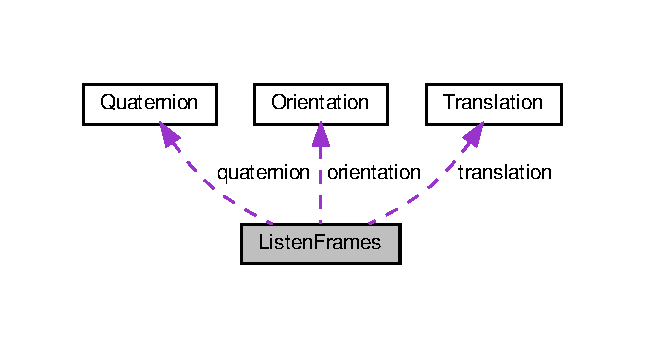
\includegraphics[width=310pt]{d2/d57/classListenFrames__coll__graph}
\end{center}
\end{figure}
\subsection*{Public Member Functions}
\begin{DoxyCompactItemize}
\item 
\mbox{\Hypertarget{classListenFrames_a33dac0513c91658e7cbbe85c0c0647cf}\label{classListenFrames_a33dac0513c91658e7cbbe85c0c0647cf}} 
void {\bfseries get\+Link\+Transform\+U\+R5} (ros\+::\+Publisher pub\+\_\+endeffector\+\_\+pose\+\_\+, const std\+::string target\+\_\+frame2)
\item 
\mbox{\Hypertarget{classListenFrames_af6e97a970ca702f7637624e4b463a56f}\label{classListenFrames_af6e97a970ca702f7637624e4b463a56f}} 
void {\bfseries get\+Pose} (ros\+::\+Publisher pub\+\_\+endeffector\+\_\+pose\+\_\+, double alpha, double beta, double gamma)
\item 
\mbox{\Hypertarget{classListenFrames_a9ba6e284adaf8241314af141a5365fff}\label{classListenFrames_a9ba6e284adaf8241314af141a5365fff}} 
void {\bfseries jacobian\+U\+R5} ()
\end{DoxyCompactItemize}
\subsection*{Public Attributes}
\begin{DoxyCompactItemize}
\item 
\mbox{\Hypertarget{classListenFrames_a19a5004b84bfd9956d292700ddb316cf}\label{classListenFrames_a19a5004b84bfd9956d292700ddb316cf}} 
double {\bfseries pose\+\_\+endeffector} \mbox{[}P\+O\+S\+E\+\_\+\+A\+R\+R\+A\+Y\+\_\+\+S\+I\+ZE\mbox{]}
\item 
\mbox{\Hypertarget{classListenFrames_ac53f0f922d4afaa280aa0095bcbe0d3f}\label{classListenFrames_ac53f0f922d4afaa280aa0095bcbe0d3f}} 
double {\bfseries pp}
\item 
\mbox{\Hypertarget{classListenFrames_a3bc61a57c7dec9d8aea5287358dcacef}\label{classListenFrames_a3bc61a57c7dec9d8aea5287358dcacef}} 
\hyperlink{structOrientation}{Orientation} {\bfseries orientation}
\item 
\mbox{\Hypertarget{classListenFrames_a6deeb6697d3c32c05243bb987c1e9c5f}\label{classListenFrames_a6deeb6697d3c32c05243bb987c1e9c5f}} 
\hyperlink{structTranslation}{Translation} {\bfseries translation}
\item 
\mbox{\Hypertarget{classListenFrames_a0ceb155e09d7d28fcce7c825bc10f99c}\label{classListenFrames_a0ceb155e09d7d28fcce7c825bc10f99c}} 
\hyperlink{structQuaternion}{Quaternion} {\bfseries quaternion}
\end{DoxyCompactItemize}


The documentation for this class was generated from the following file\+:\begin{DoxyCompactItemize}
\item 
mur\+\_\+kinematics/src/listen\+\_\+frames.\+cpp\end{DoxyCompactItemize}

\hypertarget{classmove__compliant_1_1MoveMir}{}\doxysection{move\+\_\+compliant\+::Move\+Mir Class Reference}
\label{classmove__compliant_1_1MoveMir}\index{move\_compliant::MoveMir@{move\_compliant::MoveMir}}
\doxysubsection*{Public Member Functions}
\begin{DoxyCompactItemize}
\item 
\mbox{\Hypertarget{classmove__compliant_1_1MoveMir_a5d98dfc7d3a798dea0a396156ff8a167}\label{classmove__compliant_1_1MoveMir_a5d98dfc7d3a798dea0a396156ff8a167}} 
\mbox{\hyperlink{classmove__compliant_1_1MoveMir_a5d98dfc7d3a798dea0a396156ff8a167}{Move\+Mir}} ()
\begin{DoxyCompactList}\small\item\em Constructs a new Move Mir object. \end{DoxyCompactList}\item 
\mbox{\Hypertarget{classmove__compliant_1_1MoveMir_a296aaceb81a91e41041d3348fbdfffd6}\label{classmove__compliant_1_1MoveMir_a296aaceb81a91e41041d3348fbdfffd6}} 
\mbox{\hyperlink{classmove__compliant_1_1MoveMir_a296aaceb81a91e41041d3348fbdfffd6}{$\sim$\+Move\+Mir}} ()
\begin{DoxyCompactList}\small\item\em Destroys all objects. \end{DoxyCompactList}\item 
\mbox{\Hypertarget{classmove__compliant_1_1MoveMir_ac409d5fab19a447361cf38b3ad6387a3}\label{classmove__compliant_1_1MoveMir_ac409d5fab19a447361cf38b3ad6387a3}} 
void \mbox{\hyperlink{classmove__compliant_1_1MoveMir_ac409d5fab19a447361cf38b3ad6387a3}{lookup\+Initial\+Global\+Position}} ()
\begin{DoxyCompactList}\small\item\em service requests initial global pose of endeffector in $\sim$/base\+\_\+link \end{DoxyCompactList}\item 
\mbox{\Hypertarget{classmove__compliant_1_1MoveMir_ab0f9fcf4074b74d6ccc0995e0fa31247}\label{classmove__compliant_1_1MoveMir_ab0f9fcf4074b74d6ccc0995e0fa31247}} 
void \mbox{\hyperlink{classmove__compliant_1_1MoveMir_ab0f9fcf4074b74d6ccc0995e0fa31247}{lookup\+Initial\+Local\+Position}} ()
\begin{DoxyCompactList}\small\item\em service requests initial pose of endeffector in $\sim$/base\+\_\+link\+\_\+ur5 \end{DoxyCompactList}\item 
\mbox{\Hypertarget{classmove__compliant_1_1MoveMir_a2f3109df87f165b9d97ad70de05d6871}\label{classmove__compliant_1_1MoveMir_a2f3109df87f165b9d97ad70de05d6871}} 
void \mbox{\hyperlink{classmove__compliant_1_1MoveMir_a2f3109df87f165b9d97ad70de05d6871}{lookup\+Initial\+World\+Position}} ()
\begin{DoxyCompactList}\small\item\em service requests initial pose of endeffector in $\sim$/world \end{DoxyCompactList}\item 
\mbox{\Hypertarget{classmove__compliant_1_1MoveMir_a8568d4d4ed553944a75cfab82840a53d}\label{classmove__compliant_1_1MoveMir_a8568d4d4ed553944a75cfab82840a53d}} 
void \mbox{\hyperlink{classmove__compliant_1_1MoveMir_a8568d4d4ed553944a75cfab82840a53d}{lookup\+Initial\+Mi\+RPosition}} ()
\begin{DoxyCompactList}\small\item\em service requests initial pose of MiR in $\sim$/world \end{DoxyCompactList}\item 
virtual std\+::vector$<$ double $>$ \mbox{\hyperlink{classmove__compliant_1_1MoveMir_a9b12bc5bcb58c3396844f460a977bde1}{call\+Current\+Global\+Pose}} ()
\begin{DoxyCompactList}\small\item\em calls for global position of endeffector (inside $\sim$/base\+\_\+link) \end{DoxyCompactList}\item 
virtual std\+::vector$<$ double $>$ \mbox{\hyperlink{classmove__compliant_1_1MoveMir_a6dca098d99d126dcbcbc2d6dbdeafa75}{call\+Current\+Local\+Pose}} ()
\begin{DoxyCompactList}\small\item\em calls for current local pose of endeffector (inside $\sim$/base\+\_\+link\+\_\+ur5) \end{DoxyCompactList}\item 
virtual std\+::vector$<$ double $>$ \mbox{\hyperlink{classmove__compliant_1_1MoveMir_a5ed081371ff928bb45495e67a5dfec4e}{call\+Current\+World\+Pose}} ()
\begin{DoxyCompactList}\small\item\em calls for current global pose of MiR and endeffector (inside /world) \end{DoxyCompactList}\item 
double \mbox{\hyperlink{classmove__compliant_1_1MoveMir_a2f5ddebd43807dec81b1c00a24abacda}{normalize\+\_\+angle}} (double angle)
\begin{DoxyCompactList}\small\item\em normalizes the specified angle to be 0 to M\+\_\+\+PI \end{DoxyCompactList}\item 
void \mbox{\hyperlink{classmove__compliant_1_1MoveMir_a436d66f5d18c1912e049cf4ed46df320}{pose\+Updater}} (double force\+\_\+angle)
\begin{DoxyCompactList}\small\item\em checks about rotation of specified current force\+\_\+angle \end{DoxyCompactList}\item 
\mbox{\Hypertarget{classmove__compliant_1_1MoveMir_a30c34db7d92ef11bbea35414b9aeb544}\label{classmove__compliant_1_1MoveMir_a30c34db7d92ef11bbea35414b9aeb544}} 
void \mbox{\hyperlink{classmove__compliant_1_1MoveMir_a30c34db7d92ef11bbea35414b9aeb544}{relative\+Angle\+Updater}} ()
\begin{DoxyCompactList}\small\item\em checks current pose relation between MiR and endeffector (part of nullspace movement 1) \end{DoxyCompactList}\item 
double \mbox{\hyperlink{classmove__compliant_1_1MoveMir_a597c3ae70756872a0ccfecc0fc8304f3}{get\+Current\+Force\+Angle}} ()
\begin{DoxyCompactList}\small\item\em get the current force angle object \end{DoxyCompactList}\item 
\mbox{\Hypertarget{classmove__compliant_1_1MoveMir_a5e0517fb33bb3f0cd73645f23b2b80b9}\label{classmove__compliant_1_1MoveMir_a5e0517fb33bb3f0cd73645f23b2b80b9}} 
void \mbox{\hyperlink{classmove__compliant_1_1MoveMir_a5e0517fb33bb3f0cd73645f23b2b80b9}{rotate\+To\+Force\+Direction}} ()
\begin{DoxyCompactList}\small\item\em rotate MiR into force direction \end{DoxyCompactList}\item 
void \mbox{\hyperlink{classmove__compliant_1_1MoveMir_a5805a73c4d6d7051b69f06f96600c067}{rotate\+To\+Pose\+Direction}} (double rot\+\_\+angle)
\begin{DoxyCompactList}\small\item\em connects /robot1\+\_\+ns/arm\+\_\+cartesian\+\_\+compliance\+\_\+controller/target\+\_\+pose \end{DoxyCompactList}\item 
\mbox{\Hypertarget{classmove__compliant_1_1MoveMir_a5dbad376a64a379cc7a08e50d53e0568}\label{classmove__compliant_1_1MoveMir_a5dbad376a64a379cc7a08e50d53e0568}} 
void \mbox{\hyperlink{classmove__compliant_1_1MoveMir_a5dbad376a64a379cc7a08e50d53e0568}{move\+Straight}} ()
\begin{DoxyCompactList}\small\item\em method driving MiR straight towards force direction \end{DoxyCompactList}\item 
\mbox{\Hypertarget{classmove__compliant_1_1MoveMir_acc6454fc063d3849fa064072a88aed66}\label{classmove__compliant_1_1MoveMir_acc6454fc063d3849fa064072a88aed66}} 
void \mbox{\hyperlink{classmove__compliant_1_1MoveMir_acc6454fc063d3849fa064072a88aed66}{control\+Method1}} ()
\begin{DoxyCompactList}\small\item\em position related controller rotation and translation in parallel \end{DoxyCompactList}\item 
\mbox{\Hypertarget{classmove__compliant_1_1MoveMir_aa7b9460db81d9e56f9a7f0d49a278312}\label{classmove__compliant_1_1MoveMir_aa7b9460db81d9e56f9a7f0d49a278312}} 
void \mbox{\hyperlink{classmove__compliant_1_1MoveMir_aa7b9460db81d9e56f9a7f0d49a278312}{control\+Method2}} ()
\begin{DoxyCompactList}\small\item\em position related controller rotation and translation in sequence (nullspace movement 1) \end{DoxyCompactList}\item 
\mbox{\Hypertarget{classmove__compliant_1_1MoveMir_adbe8b3751258adf7893f483f113448ce}\label{classmove__compliant_1_1MoveMir_adbe8b3751258adf7893f483f113448ce}} 
void \mbox{\hyperlink{classmove__compliant_1_1MoveMir_adbe8b3751258adf7893f483f113448ce}{control\+Method3}} ()
\begin{DoxyCompactList}\small\item\em position related controller rotation and translation in sequence (nullspace movement 2) \end{DoxyCompactList}\end{DoxyCompactItemize}
\doxysubsection*{Protected Member Functions}
\begin{DoxyCompactItemize}
\item 
\mbox{\Hypertarget{classmove__compliant_1_1MoveMir_a1707efb46cd33aad2305254e511e9c94}\label{classmove__compliant_1_1MoveMir_a1707efb46cd33aad2305254e511e9c94}} 
void \mbox{\hyperlink{classmove__compliant_1_1MoveMir_a1707efb46cd33aad2305254e511e9c94}{wrench\+Callback}} (geometry\+\_\+msgs\+::\+Wrench\+Stamped wrench\+\_\+msg)
\begin{DoxyCompactList}\small\item\em Callbacks current wrench. \end{DoxyCompactList}\end{DoxyCompactItemize}


\doxysubsection{Member Function Documentation}
\mbox{\Hypertarget{classmove__compliant_1_1MoveMir_a9b12bc5bcb58c3396844f460a977bde1}\label{classmove__compliant_1_1MoveMir_a9b12bc5bcb58c3396844f460a977bde1}} 
\index{move\_compliant::MoveMir@{move\_compliant::MoveMir}!callCurrentGlobalPose@{callCurrentGlobalPose}}
\index{callCurrentGlobalPose@{callCurrentGlobalPose}!move\_compliant::MoveMir@{move\_compliant::MoveMir}}
\doxysubsubsection{\texorpdfstring{callCurrentGlobalPose()}{callCurrentGlobalPose()}}
{\footnotesize\ttfamily std\+::vector$<$ double $>$ Move\+Mir\+::call\+Current\+Global\+Pose (\begin{DoxyParamCaption}{ }\end{DoxyParamCaption})\hspace{0.3cm}{\ttfamily [virtual]}}

\begin{DoxyReturn}{Returns}
std\+::vector$<$double$>$ current\+\_\+pose 
\end{DoxyReturn}
\mbox{\Hypertarget{classmove__compliant_1_1MoveMir_a6dca098d99d126dcbcbc2d6dbdeafa75}\label{classmove__compliant_1_1MoveMir_a6dca098d99d126dcbcbc2d6dbdeafa75}} 
\index{move\_compliant::MoveMir@{move\_compliant::MoveMir}!callCurrentLocalPose@{callCurrentLocalPose}}
\index{callCurrentLocalPose@{callCurrentLocalPose}!move\_compliant::MoveMir@{move\_compliant::MoveMir}}
\doxysubsubsection{\texorpdfstring{callCurrentLocalPose()}{callCurrentLocalPose()}}
{\footnotesize\ttfamily std\+::vector$<$ double $>$ Move\+Mir\+::call\+Current\+Local\+Pose (\begin{DoxyParamCaption}{ }\end{DoxyParamCaption})\hspace{0.3cm}{\ttfamily [virtual]}}

\begin{DoxyReturn}{Returns}
std\+::vector$<$double$>$ current\+\_\+pose 
\end{DoxyReturn}
\mbox{\Hypertarget{classmove__compliant_1_1MoveMir_a5ed081371ff928bb45495e67a5dfec4e}\label{classmove__compliant_1_1MoveMir_a5ed081371ff928bb45495e67a5dfec4e}} 
\index{move\_compliant::MoveMir@{move\_compliant::MoveMir}!callCurrentWorldPose@{callCurrentWorldPose}}
\index{callCurrentWorldPose@{callCurrentWorldPose}!move\_compliant::MoveMir@{move\_compliant::MoveMir}}
\doxysubsubsection{\texorpdfstring{callCurrentWorldPose()}{callCurrentWorldPose()}}
{\footnotesize\ttfamily std\+::vector$<$ double $>$ Move\+Mir\+::call\+Current\+World\+Pose (\begin{DoxyParamCaption}{ }\end{DoxyParamCaption})\hspace{0.3cm}{\ttfamily [virtual]}}

\begin{DoxyReturn}{Returns}
std\+::vector$<$double$>$ current\+\_\+map\+\_\+pose\+\_\+, std\+::vector$<$double$>$ current\+\_\+mir\+\_\+map\+\_\+pose\+\_\+ 
\end{DoxyReturn}
\mbox{\Hypertarget{classmove__compliant_1_1MoveMir_a597c3ae70756872a0ccfecc0fc8304f3}\label{classmove__compliant_1_1MoveMir_a597c3ae70756872a0ccfecc0fc8304f3}} 
\index{move\_compliant::MoveMir@{move\_compliant::MoveMir}!getCurrentForceAngle@{getCurrentForceAngle}}
\index{getCurrentForceAngle@{getCurrentForceAngle}!move\_compliant::MoveMir@{move\_compliant::MoveMir}}
\doxysubsubsection{\texorpdfstring{getCurrentForceAngle()}{getCurrentForceAngle()}}
{\footnotesize\ttfamily double Move\+Mir\+::get\+Current\+Force\+Angle (\begin{DoxyParamCaption}{ }\end{DoxyParamCaption})}

\begin{DoxyReturn}{Returns}
double force\+\_\+angle ~\newline
 
\end{DoxyReturn}
\mbox{\Hypertarget{classmove__compliant_1_1MoveMir_a2f5ddebd43807dec81b1c00a24abacda}\label{classmove__compliant_1_1MoveMir_a2f5ddebd43807dec81b1c00a24abacda}} 
\index{move\_compliant::MoveMir@{move\_compliant::MoveMir}!normalize\_angle@{normalize\_angle}}
\index{normalize\_angle@{normalize\_angle}!move\_compliant::MoveMir@{move\_compliant::MoveMir}}
\doxysubsubsection{\texorpdfstring{normalize\_angle()}{normalize\_angle()}}
{\footnotesize\ttfamily double Move\+Mir\+::normalize\+\_\+angle (\begin{DoxyParamCaption}\item[{double}]{angle }\end{DoxyParamCaption})}


\begin{DoxyParams}{Parameters}
{\em angle} & \\
\hline
\end{DoxyParams}
\begin{DoxyReturn}{Returns}
double normalized\+\_\+angle 
\end{DoxyReturn}
\mbox{\Hypertarget{classmove__compliant_1_1MoveMir_a436d66f5d18c1912e049cf4ed46df320}\label{classmove__compliant_1_1MoveMir_a436d66f5d18c1912e049cf4ed46df320}} 
\index{move\_compliant::MoveMir@{move\_compliant::MoveMir}!poseUpdater@{poseUpdater}}
\index{poseUpdater@{poseUpdater}!move\_compliant::MoveMir@{move\_compliant::MoveMir}}
\doxysubsubsection{\texorpdfstring{poseUpdater()}{poseUpdater()}}
{\footnotesize\ttfamily void Move\+Mir\+::pose\+Updater (\begin{DoxyParamCaption}\item[{double}]{force\+\_\+angle }\end{DoxyParamCaption})}


\begin{DoxyParams}{Parameters}
{\em force\+\_\+angle} & \\
\hline
\end{DoxyParams}
\mbox{\Hypertarget{classmove__compliant_1_1MoveMir_a5805a73c4d6d7051b69f06f96600c067}\label{classmove__compliant_1_1MoveMir_a5805a73c4d6d7051b69f06f96600c067}} 
\index{move\_compliant::MoveMir@{move\_compliant::MoveMir}!rotateToPoseDirection@{rotateToPoseDirection}}
\index{rotateToPoseDirection@{rotateToPoseDirection}!move\_compliant::MoveMir@{move\_compliant::MoveMir}}
\doxysubsubsection{\texorpdfstring{rotateToPoseDirection()}{rotateToPoseDirection()}}
{\footnotesize\ttfamily void Move\+Mir\+::rotate\+To\+Pose\+Direction (\begin{DoxyParamCaption}\item[{double}]{rot\+\_\+angle }\end{DoxyParamCaption})}


\begin{DoxyParams}{Parameters}
{\em rot\+\_\+angle} & angle between Mi\+R-\/x-\/axis and target direction \\
\hline
\end{DoxyParams}


The documentation for this class was generated from the following files\+:\begin{DoxyCompactItemize}
\item 
mur\+\_\+force\+\_\+controller/include/mur\+\_\+force\+\_\+controller/move\+\_\+mir\+\_\+compliant.\+h\item 
mur\+\_\+force\+\_\+controller/src/move\+\_\+mir\+\_\+compliant.\+cpp\end{DoxyCompactItemize}

\hypertarget{classmove__compliant_1_1MurBase}{}\section{move\+\_\+compliant\+:\+:Mur\+Base Class Reference}
\label{classmove__compliant_1_1MurBase}\index{move\+\_\+compliant\+::\+Mur\+Base@{move\+\_\+compliant\+::\+Mur\+Base}}


base class ready to get inherited  




{\ttfamily \#include $<$move\+\_\+compliant.\+h$>$}



Inheritance diagram for move\+\_\+compliant\+:\+:Mur\+Base\+:
\nopagebreak
\begin{figure}[H]
\begin{center}
\leavevmode
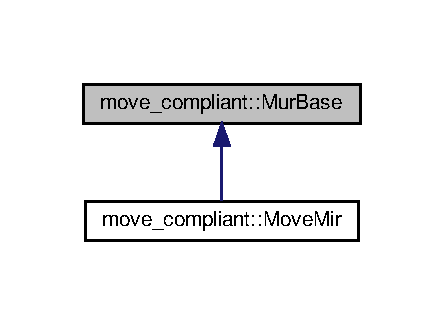
\includegraphics[width=213pt]{d4/d55/classmove__compliant_1_1MurBase__inherit__graph}
\end{center}
\end{figure}
\subsection*{Public Member Functions}
\begin{DoxyCompactItemize}
\item 
\mbox{\Hypertarget{classmove__compliant_1_1MurBase_a3ca7696f5ee13563dabe58e6502f9dbf}\label{classmove__compliant_1_1MurBase_a3ca7696f5ee13563dabe58e6502f9dbf}} 
virtual void \hyperlink{classmove__compliant_1_1MurBase_a3ca7696f5ee13563dabe58e6502f9dbf}{callback\+Joint\+Angles} (sensor\+\_\+msgs\+::\+Joint\+State joint\+\_\+msg)
\begin{DoxyCompactList}\small\item\em callback function of joints data \end{DoxyCompactList}\end{DoxyCompactItemize}


The documentation for this class was generated from the following files\+:\begin{DoxyCompactItemize}
\item 
mur\+\_\+force\+\_\+controller/include/mur\+\_\+force\+\_\+controller/move\+\_\+compliant.\+h\item 
mur\+\_\+force\+\_\+controller/src/move\+\_\+compliant.\+cpp\end{DoxyCompactItemize}

\hypertarget{structOrientation}{}\section{Orientation Struct Reference}
\label{structOrientation}\index{Orientation@{Orientation}}
\subsection*{Public Attributes}
\begin{DoxyCompactItemize}
\item 
\mbox{\Hypertarget{structOrientation_a5afb9011203e023f5191b5512a1b5393}\label{structOrientation_a5afb9011203e023f5191b5512a1b5393}} 
double {\bfseries x}
\item 
\mbox{\Hypertarget{structOrientation_a799925b012c217b99ced1e8d67ce8fac}\label{structOrientation_a799925b012c217b99ced1e8d67ce8fac}} 
double {\bfseries y}
\item 
\mbox{\Hypertarget{structOrientation_a5868530129dc0877d517a3a92074a79a}\label{structOrientation_a5868530129dc0877d517a3a92074a79a}} 
double {\bfseries z}
\end{DoxyCompactItemize}


The documentation for this struct was generated from the following file\+:\begin{DoxyCompactItemize}
\item 
mur\+\_\+kinematics/src/listen\+\_\+frames.\+cpp\end{DoxyCompactItemize}

\hypertarget{structQuaternion}{}\section{Quaternion Struct Reference}
\label{structQuaternion}\index{Quaternion@{Quaternion}}
\subsection*{Public Attributes}
\begin{DoxyCompactItemize}
\item 
\mbox{\Hypertarget{structQuaternion_a65c93d8db6c57203447bd0594b608512}\label{structQuaternion_a65c93d8db6c57203447bd0594b608512}} 
double {\bfseries x}
\item 
\mbox{\Hypertarget{structQuaternion_acfea23e3ba2b57356fe36b4d8f4c52f3}\label{structQuaternion_acfea23e3ba2b57356fe36b4d8f4c52f3}} 
double {\bfseries y}
\item 
\mbox{\Hypertarget{structQuaternion_a90bbdb05526bddfbc3247dcc9a5cace4}\label{structQuaternion_a90bbdb05526bddfbc3247dcc9a5cace4}} 
double {\bfseries z}
\item 
\mbox{\Hypertarget{structQuaternion_aeded08fcb4e8d0866e612ed81cb44aa7}\label{structQuaternion_aeded08fcb4e8d0866e612ed81cb44aa7}} 
double {\bfseries w}
\end{DoxyCompactItemize}


The documentation for this struct was generated from the following file\+:\begin{DoxyCompactItemize}
\item 
mur\+\_\+kinematics/src/listen\+\_\+frames.\+cpp\end{DoxyCompactItemize}

\hypertarget{structTranslation}{}\section{Translation Struct Reference}
\label{structTranslation}\index{Translation@{Translation}}
\subsection*{Public Attributes}
\begin{DoxyCompactItemize}
\item 
\mbox{\Hypertarget{structTranslation_a7b3aea7b8380a81367a7c289b7a19af7}\label{structTranslation_a7b3aea7b8380a81367a7c289b7a19af7}} 
double {\bfseries x}
\item 
\mbox{\Hypertarget{structTranslation_a4080bcfcd8dc16dd59d8e126a4cf3763}\label{structTranslation_a4080bcfcd8dc16dd59d8e126a4cf3763}} 
double {\bfseries y}
\item 
\mbox{\Hypertarget{structTranslation_ac87bf35effcf1ab42669b2f6b1d0c0db}\label{structTranslation_ac87bf35effcf1ab42669b2f6b1d0c0db}} 
double {\bfseries z}
\end{DoxyCompactItemize}


The documentation for this struct was generated from the following file\+:\begin{DoxyCompactItemize}
\item 
mur\+\_\+kinematics/src/listen\+\_\+frames.\+cpp\end{DoxyCompactItemize}

\hypertarget{classWrenchPublisher}{}\section{Wrench\+Publisher Class Reference}
\label{classWrenchPublisher}\index{Wrench\+Publisher@{Wrench\+Publisher}}
\subsection*{Classes}
\begin{DoxyCompactItemize}
\item 
struct \hyperlink{structWrenchPublisher_1_1Frames}{Frames}
\end{DoxyCompactItemize}
\subsection*{Public Member Functions}
\begin{DoxyCompactItemize}
\item 
\mbox{\Hypertarget{classWrenchPublisher_a418dba02ad920b09c1b3948750a2934d}\label{classWrenchPublisher_a418dba02ad920b09c1b3948750a2934d}} 
void \hyperlink{classWrenchPublisher_a418dba02ad920b09c1b3948750a2934d}{wrench\+Callback} (geometry\+\_\+msgs\+::\+Wrench\+Stamped\+::\+Const\+Ptr wrench\+\_\+msg)
\begin{DoxyCompactList}\small\item\em Callbacks current wrench and publishes it to cartesian\+\_\+admittance\+\_\+controller. \end{DoxyCompactList}\item 
\mbox{\Hypertarget{classWrenchPublisher_a2364056bf9eaa8dfc7d4021107c89e10}\label{classWrenchPublisher_a2364056bf9eaa8dfc7d4021107c89e10}} 
void \hyperlink{classWrenchPublisher_a2364056bf9eaa8dfc7d4021107c89e10}{transform\+\_\+wrench\+\_\+into\+\_\+ee} ()
\begin{DoxyCompactList}\small\item\em transfers current wrench of Gazebo-\/\+F/\+T-\/sensor-\/plugin fixed at \textquotesingle{}wrist3\+\_\+link\+\_\+ur5\textquotesingle{} into \textquotesingle{}ee\+\_\+link\+\_\+ur5\textquotesingle{} \end{DoxyCompactList}\end{DoxyCompactItemize}


The documentation for this class was generated from the following files\+:\begin{DoxyCompactItemize}
\item 
mur\+\_\+simulation/include/mur\+\_\+simulation/gazebo\+\_\+ft\+\_\+publisher.\+h\item 
mur\+\_\+simulation/src/gazebo\+\_\+ft\+\_\+publisher.\+cpp\end{DoxyCompactItemize}

%--- End generated contents ---

% Index
\backmatter
\newpage
\phantomsection
\clearemptydoublepage
\addcontentsline{toc}{chapter}{Index}
\printindex

\end{document}
